\documentclass[11pt,letterpaper]{exam}
\usepackage[latin1]{inputenc}
\usepackage[left=3.00cm, right=3.00cm, top=3.00cm, bottom=3.00cm]{geometry}% You can change margins here
\usepackage{amsmath}
\usepackage{amsthm}
\usepackage[]{algorithm2e}
\usepackage{amssymb} % use for therefore
\usepackage{tabto}
\usepackage{gensymb}
\usepackage{graphicx} % resize table
\usepackage{listings}

\author{Elvric Trombert\\260673394\\Simon Zheng\\260744353}% Put your Student ID here
\title{Assignment 1 ECSE 420}
\date{October $10^{\textnormal{th}}$, 2018}
\begin{document}
	\maketitle
	\header{}{Assignment 1 ECSE 420}{}
	\hrulefill
	\begin{questions}
		\question
		    \section*{Matrix Multiplication}
		    \subsection*{1.4., 1.5. \& 1.6.}
			These tests were ran using MatrixMultiplication.java file in the ca.mcgill.ecse420.a1 package which was given to us at the start of the assignment. The number of threads and matrix size was hard coded each time in the class private variables the code was then compile and run each time to generate the data bellow.
			\begin{figure}[h!]
				\centering
				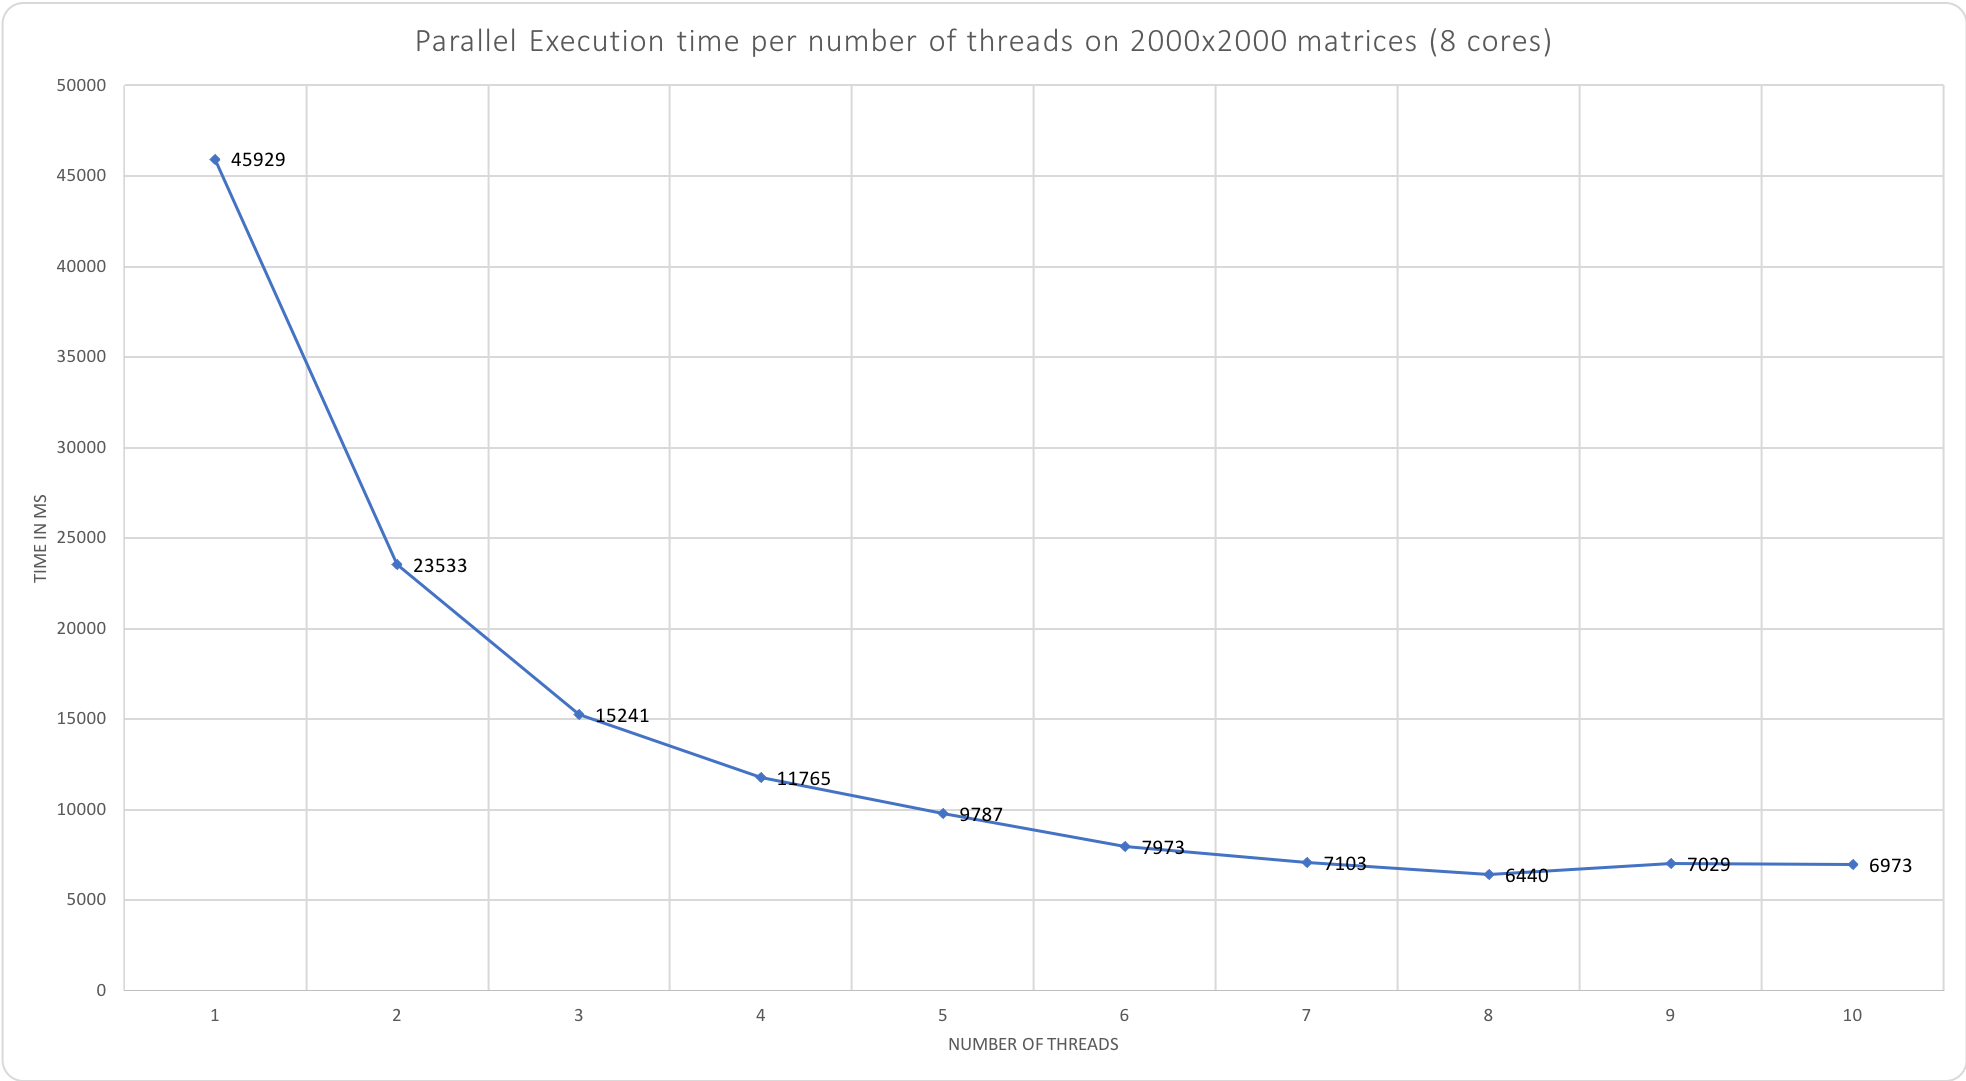
\includegraphics[scale=0.5]{ExecutionTimeThread}
			\end{figure}
			This graph follows an exponential decrease in resolution time as we increase the number of threads. It is important to note that we run this test on a 8 core CPU machine. The reason for that exponential decrease is that at first the amount of work done by a single thread for a matrix size x becomes x/2 then x/3 and so on. The size of the region that each thread needs to calculate decreases by a smaller and smaller ratio compare to the previous size every time we add a new thread. This is why the decrease in running time is exponential as the size calculated by each thread decreases by a smaller amount each time until the number of threads equals the number of cores.

			\quad Since we are running on an 8 core machine it is normal to see a slight increase in running time when the number of threads exceeds the number of cores as this adds overhead cost when switching between threads. In our case this was observed for 9 threads however for 10 threads the execution time decreased compare to the one with 9 threads. We think that this may be due to the fact that the execution region of each thread became so small with 10 threads that most thread managed to finish before the hardware algorithm asked for an other thread to get CPU runtime which reduced overhead switch cost as it did not need to load the interrupted thread back on the CPU again after the swap.
			\begin{figure}[h!]
				\centering
				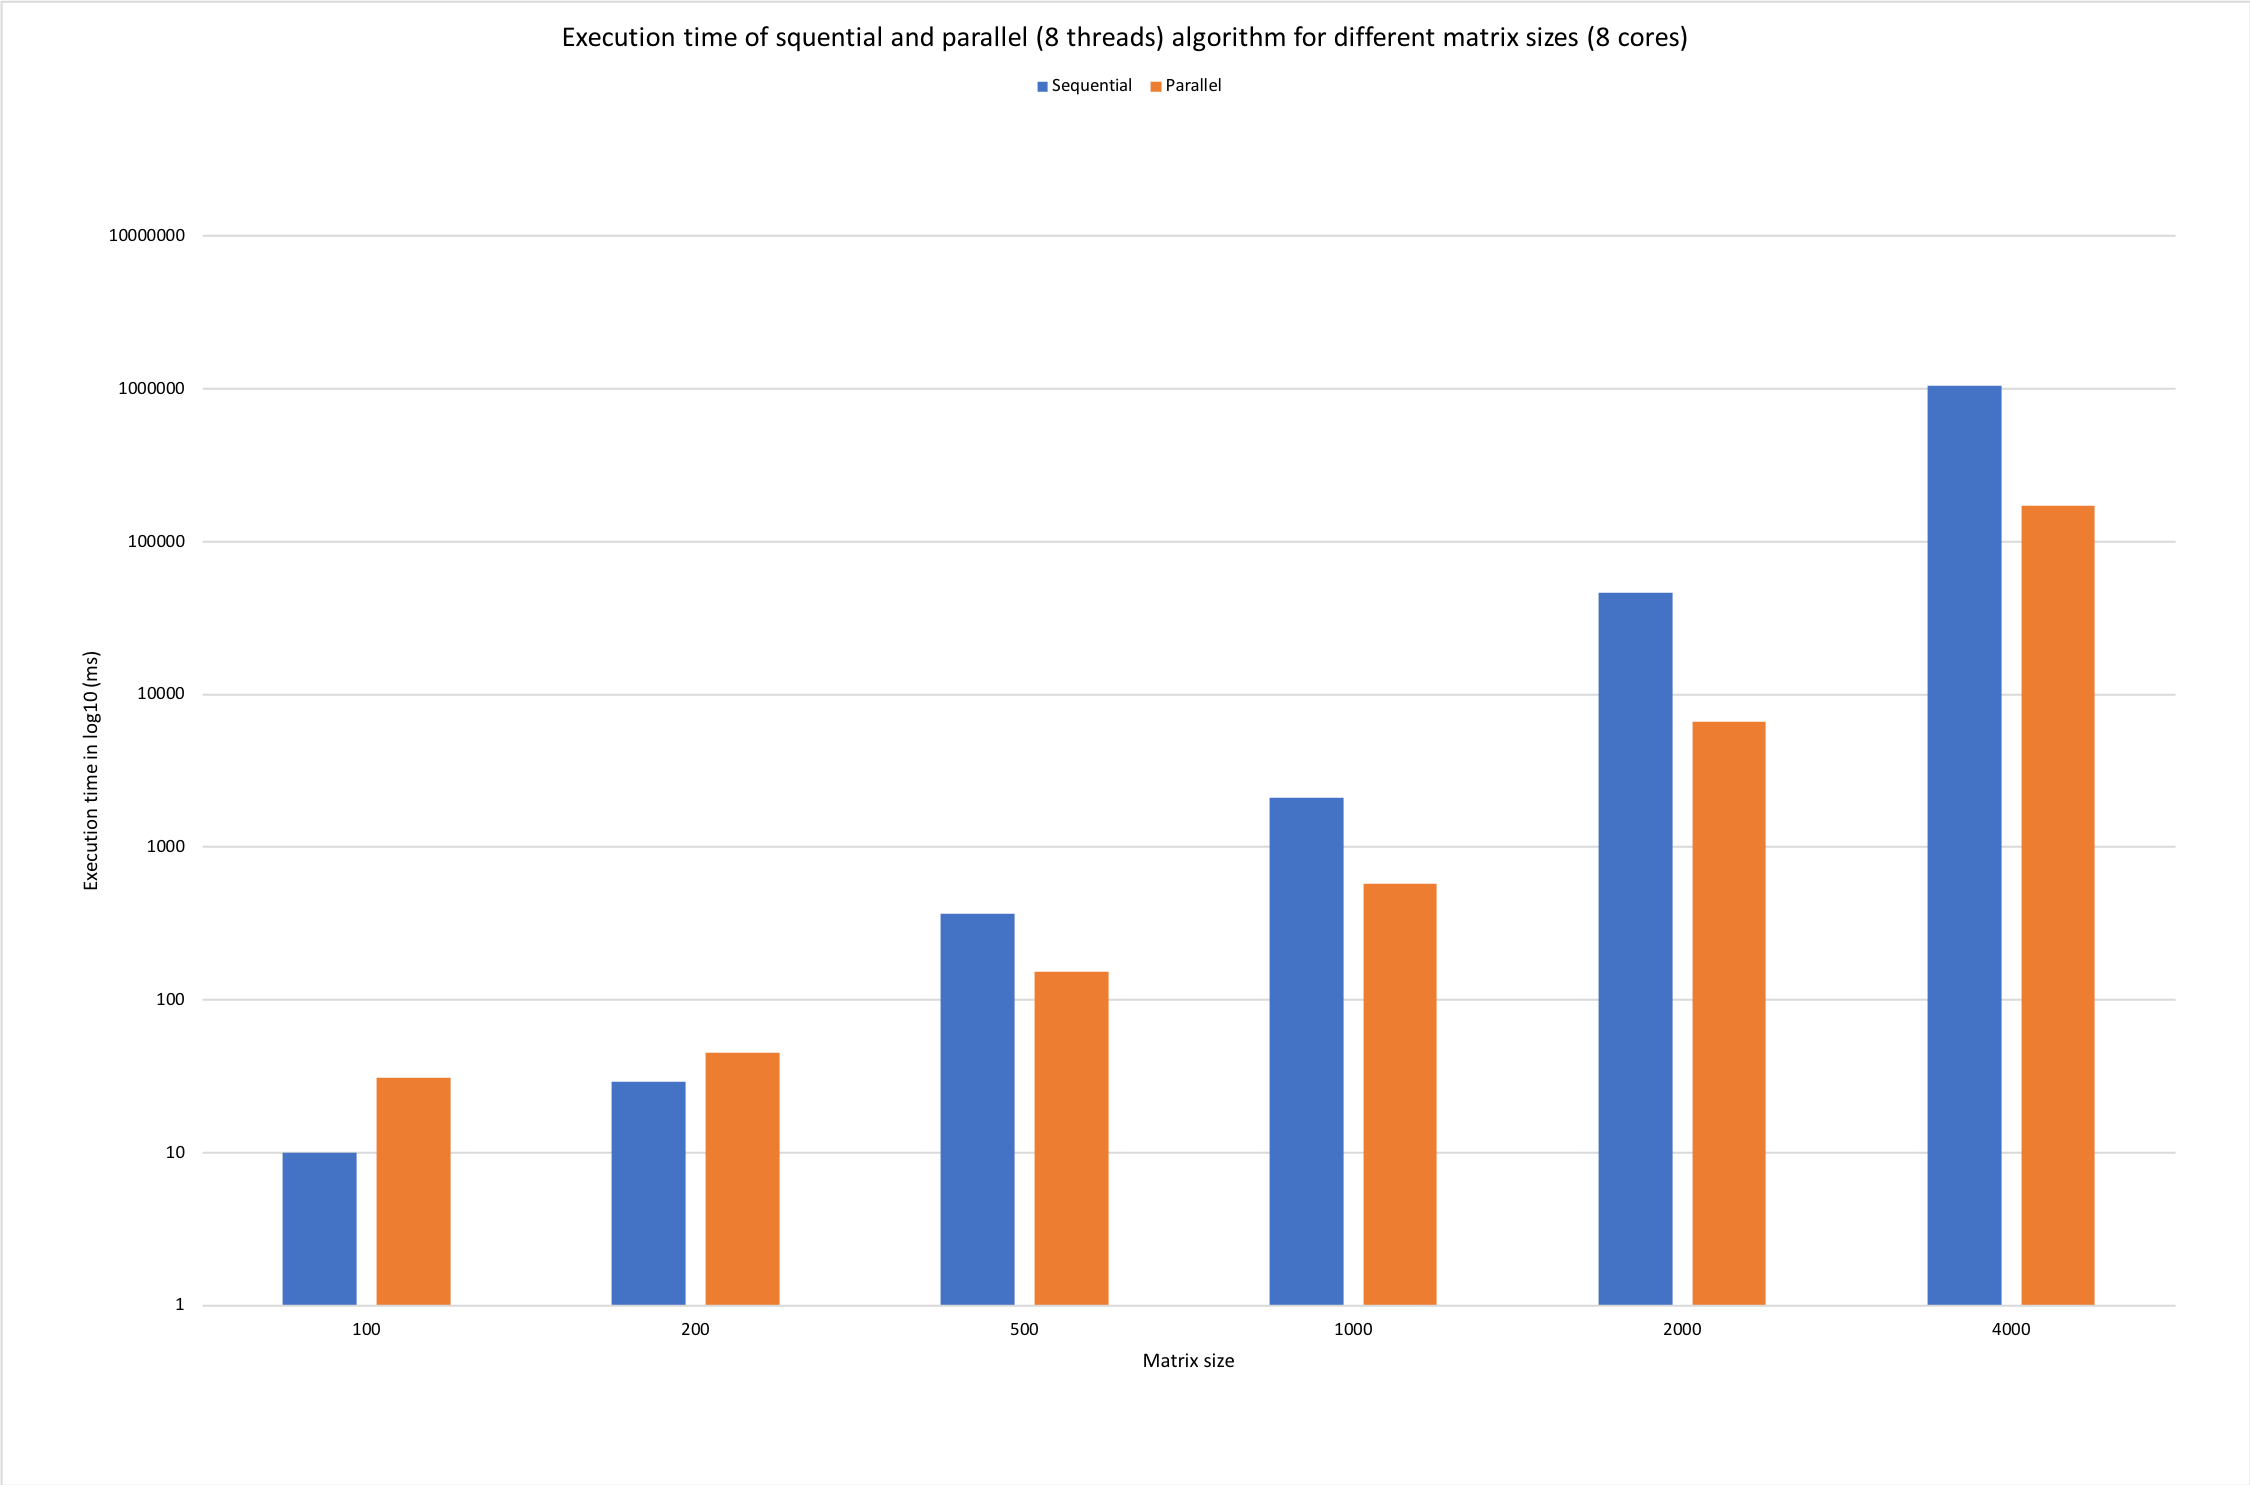
\includegraphics[scale=0.4]{ExectionParallelSequential}
			\end{figure}

			In this case we decided to graph the results on a log scale as the execution time difference between matrix size 100 and 4000 was too large to be visualized on a normal scale. Here the execution time followed a exponential increase for both parallel and sequential as we double the size of the matrix on every tries but had the same number of threads on every try. In this case we can see that the execution time of sequential matrix multiplication performed better than the parallel for size 100 and 200 (note that we tried to use 1 to 8 threads for parallel and all times where worse than sequential for all combination at these matrix sizes). We think this is due to the time required to instantiate the executor and the parallelMultiplication class for parallel that adds greater overheads than just directly starting the sequential execution. However the costs of these overheads becomes negligible as soon as the matrix size goes over 200 the extra computational power given by the threads becomes more important.

        \newpage

		\question
		    \section*{Deadlock questions}
			The deadlock java file is in the package ca.mcgill.ecse420.a1 named: Deadlocker.java.
			Here is a sample output of the program:\\
			New attempt...\\
			Thread 1 started\\
			Thread 1 waits to acquire lock 0\\
			Thread 1 acquired lock 0\\
			Thread 2 started\\
			Thread 1 sleeps for 694 milliseconds\\
			Thread 2 sleeps for 986 milliseconds\\
			Thread 1 waits to acquire lock 1\\
			Thread 1 acquired lock 1\\
			Thread 1 unlocked both locks\\
			Thread 1 terminated\\
			Thread 2 waits to acquire lock 1\\
			Thread 2 acquired lock 1\\
			Thread 2 waits to acquire lock 0\\
			Thread 2 acquired lock 0\\
			Thread 2 unlocked both locks\\
			Thread 2 terminated\\
			New attempt...\\
			Thread 1 started\\
			Thread 1 waits to acquire lock 0\\
			Thread 2 started\\
			Thread 1 acquired lock 0\\
			Thread 2 sleeps for 42 milliseconds\\
			Thread 1 sleeps for 919 milliseconds\\
			Thread 2 waits to acquire lock 1\\
			Thread 2 acquired lock 1\\
			Thread 2 waits to acquire lock 0\\
			Thread 1 waits to acquire lock 1\\
			\begin{parts}
				\part
				    \subsection*{2.1. Explain under what conditions a deadlock could happen.}
					In our case deadlock can occur when the sleep time of Thread 1 is longer than than the sleep time of Thread 2. Since Thread 1 would have acquired lock 0 but will not be able to acquire lock 1. As it would have been acquired by Thread 2 who will be waiting for lock 0 already held by thread 1. Hence we are in a deadlock as neither Thread is willing to give up their resources but cannot finish their execution without the other thread's resources.
				\part
				    \subsection*{2.2. Discuss possible design solutions to avoid deadlock.}
					Hold-and-wait

					Require a thread to request all of its required resources at a time making it block otherwise only activating it when all the resources are available. This prohibits resources from being use optimally. Sometimes it is hard to know in advance all the resources that a thread will need and certain resources might either be use after a long time laps or not even used at all.

					No preemption

					If a thread holding resources is denied a further request that thread must release all its unused resources and ask for them again. This could be applied to the code we used to illustrate the deadlock example. However the issue with this would be that the thread may have to loop for a long time to acquire all of its required resources.

					Circular wait

					Can be prevented by defining a linear ordering of resource type. If a thread has been allocated resource of type R, then it may subsequently request only those resources of types following R in the ordering. So T1 holds are R1 it can only request $Ri>1$, T2 holds R2 so it can only request $Ri>2$.
			\end{parts}

		\newpage

		\question
		\section*{Dining Philosophers}
		The dining philosopher files are DiningPhilosopher.java and DiningPhilosopherSync.java in the ca.mcgill.ecse420.a1 package for respectively the deadlocking version and deadlock-free + starvation-free version.
		\subsection*{3.1. \& 3.2. Explain your solution to avoid deadlock and starvation.}
		Our solution was to only allow $n-1$ philosophers at most to eat simultaneously, where $n =$ number of chopsticks $=$ number of philosophers.

		The way it works is that when a philosopher goes to pick up a chopstick, if there is already n-1 other philosophers eating, he will wait instead (this can be thought of as him returning to thinking). Thus, we avoid a deadlock.

		In terms of actual implementation, and keeping it starvation-free, the important things are that the locks themselves are fair. When a philosopher object (thread) goes to pick up their chopsticks, we use a \textit{fair} mutex (ReentrantLock with the "true" argument) to lock all the chopsticks and a condition ($\le n-1$ philosophers already eating) that tells the thread/philosopher whether to proceed (condition respected) or wait his turn before unlocking the mutex.

		If he must wait, then he calls await() on the condition inside the mutex (critical section) to wait.
		If he is done eating, then he calls signal() inside the critical section to signal the next philosopher "in line" (because the mutex lock is fair) to pick up his chopsticks start eating.

		The number of philosophers eating is kept track of by a global counter whose mutation is protected by the mutex.
		When entering the critical section through the mutex to eat, it is incremented, and when doing the same after being done eating, it is decremented.

		When a philosopher can finally pick up his chopsticks, he locks the "chopsticks" which are themselves fair ReentrantLocks.

		This way, it stops deadlocks from happening (deadlock-free) and keeps things fair/starvation-free.

		\subsection*{Output example}

		\begin{lstlisting}
Philosopher #0 created.
Philosopher #1 created.
Philosopher #2 created.
Philosopher #3 created.
Philosopher #4 created.
Philosopher #1 started running.
Philosopher #2 started running.
Philosopher #0 started running.
Philosopher #4 started running.
Philosopher #3 started running.
Philosopher #1 eating. Average wait time (ns): 32386 and ate 1 times.
Philosopher #0 eating. Average wait time (ns): 25358875 and ate 1 times.
Philosopher #2 eating. Average wait time (ns): 25417992 and ate 1 times.
Philosopher #4 eating. Average wait time (ns): 25390233 and ate 1 times.
Philosopher #0 thinking.
Philosopher #3 eating. Average wait time (ns): 25629783 and ate 1 times.
Philosopher #2 thinking.
Philosopher #4 thinking.
Philosopher #1 thinking.
Philosopher #3 thinking.
Philosopher #0 eating. Average wait time (ns): 12682265 and ate 2 times.
Philosopher #2 eating. Average wait time (ns): 12711566 and ate 2 times.
Philosopher #2 thinking.
Philosopher #4 eating. Average wait time (ns): 12795614 and ate 2 times.
Philosopher #0 thinking.
Philosopher #3 eating. Average wait time (ns): 12954714 and ate 2 times.
Philosopher #3 thinking.
Philosopher #4 thinking.
Philosopher #1 eating. Average wait time (ns): 113349 and ate 2 times.
Philosopher #1 thinking.
...
Philosopher #1 eating. Average wait time (ns): 41920 and ate 9045437 times.
Philosopher #0 eating. Average wait time (ns): 44903 and ate 8496381 times.
Philosopher #0 thinking.
Philosopher #4 eating. Average wait time (ns): 43917 and ate 8563114 times.
Philosopher #1 thinking.
Philosopher #3 eating. Average wait time (ns): 47470 and ate 8140978 times.
Philosopher #4 thinking.
Philosopher #2 eating. Average wait time (ns): 46074 and ate 8105521 times.
Philosopher #2 thinking.
Philosopher #2 eating. Average wait time (ns): 46074 and ate 8105522 times.
Philosopher #2 thinking.
Philosopher #2 eating. Average wait time (ns): 46074 and ate 8105523 times.
Philosopher #2 thinking.
Philosopher #2 eating. Average wait time (ns): 46074 and ate 8105524 times.
Philosopher #2 thinking.
Philosopher #2 eating. Average wait time (ns): 46074 and ate 8105525 times.
Philosopher #2 thinking.
Philosopher #2 eating. Average wait time (ns): 46074 and ate 8105526 times.
Philosopher #3 thinking.
Philosopher #0 eating. Average wait time (ns): 44903 and ate 8496382 times.
Philosopher #0 thinking.
Philosopher #1 eating. Average wait time (ns): 41920 and ate 9045438 times.
Philosopher #2 thinking.
Philosopher #1 thinking.
Philosopher #4 eating. Average wait time (ns): 43917 and ate 8563115 times.
		\end{lstlisting}

		\newpage

		\question
		\section*{Amdahl's Law}
		Amdahl's law = $s = \frac{1}{1-p+\frac{p}{N}}$
		Where s is the speed up and N the number of processors/threads.
			\begin{parts}
				\part
				    \subsection*{4.1. Find a limit for the overall speedup that can be achieved by
running the program on a multiprocessor machine.}
					The sequential part of a program takes 40\% on a single processor remains the same on multi processor as it cannot be parallelized. Hence to get the speed up limit we get the following equation
					\begin{align*}
						s &= \frac{1}{0.4+\frac{0.6}{\infty}}\\
						s &= \frac{1}{0.4}\\
						&= 2.5
					\end{align*}
				\part
				    \subsection*{4.2. What value of k should you require?}
					$a=\frac{1}{k}$
					\begin{align*}
						2s_n &= \frac{2}{0.2+\frac{0.8}{n}}\\
						2s_n &= \frac{1}{0.2a+\frac{1-0.2a}{n}}\\
						\therefore \frac{2}{0.2+\frac{0.8}{n}} &= \frac{1}{0.2a+\frac{1-0.2a}{n}}\\
						0.4a+\frac{2-0.4a}{n} &= 0.2+\frac{0.8}{n}\\
						0.4an+2-0.4a &= 0.2n+0.8\\
						0.4a(n-1) &= 0.2n-1.2\\
						\therefore a &< \frac{0.2n-1.2}{0.4(n-1)}\\
						a &< \frac{n-6}{2(n-1)}\\
						\therefore k &> \frac{2(n-1)}{n-6}, n>6
					\end{align*}

				\part
				    \subsection*{4.3. What fraction of the overall execution time did the sequential part account for? Express your
answer as a function of n.}
					$s_p=$ speed up for $s/3$, $s=$ sequential time
					\begin{align*}
						s_p &= \frac{2}{s+\frac{1-s}{n}}\\
						s_p &= \frac{1}{\frac{s}{3}+\frac{1-\frac{s}{3}}{n}}\\
						\therefore \frac{2}{s+\frac{1-s}{n}} &= \frac{1}{\frac{s}{3}+\frac{1-\frac{s}{3}}{n}}\\
						\frac{2s}{3}+\frac{2-\frac{2s}{3}}{n} &= s+\frac{1-s}{n}\\
						\frac{2sn}{3}+2-\frac{2s}{3} &= sn+1-s\\
						1 &= \frac{sn}{3}-\frac{s}{3}\\
						1 &= \frac{s}{3}(n-1)\\
						s &= \frac{3}{n-1}, n > 4
					\end{align*}
			\end{parts}
	\end{questions}

	\newpage

	\section*{Appendix}

\subsection*{MatrixMultiplication.java}
\begin{lstlisting}
package ca.mcgill.ecse420.a1;

import java.util.concurrent.ExecutorService;
import java.util.concurrent.Executors;

public class MatrixMultiplication {

  private static final int NUMBER_THREADS = 2;
  private static final int MATRIX_SIZE = 2000;

  // To make it easier to use inside the nested ParallelMatrixMultiplication class
  protected static double[][] a;
  protected static double[][] b;

  public static void main(String[] args) {

    // Generate two random matrices, same size
    MatrixMultiplication.a = generateRandomMatrix(MATRIX_SIZE, MATRIX_SIZE);
    MatrixMultiplication.b = generateRandomMatrix(MATRIX_SIZE, MATRIX_SIZE);
    measureSequentialTime();
    measureParallelTime();
  }

  public static void measureSequentialTime() {
    long startTime = System.currentTimeMillis();
    sequentialMultiplyMatrix(a, b);
    long endTime = System.currentTimeMillis();
    long runTime = endTime - startTime;
    System.out.println("Runtime (sequential) : " + runTime);
  }

  public static void measureParallelTime() {
    long startTime = System.currentTimeMillis();
    parallelMultiplyMatrix(a, b);
    long endTime = System.currentTimeMillis();
    long runTime = endTime - startTime;
    System.out.println("Runtime (parallel) : " + runTime);
  }

  /**
   * Returns the result of a sequential matrix multiplication The two matrices are randomly
   * generated
   *
   * @param a is the first matrix
   * @param b is the second matrix
   * @return the result of the multiplication
   */
  public static double[][] sequentialMultiplyMatrix(double[][] a, double[][] b) {
    double[][] result = new double[MATRIX_SIZE][MATRIX_SIZE];
    for (int i = 0; i < MATRIX_SIZE; i++) {
      for (int j = 0; j < MATRIX_SIZE; j++) {
        for (int k = 0; k < MATRIX_SIZE; k++) {
          result[i][j] += a[i][k] * b[k][j];
        }
      }
    }
    return result;
  }

  /**
   * Returns the result of a concurrent matrix multiplication The two matrices are randomly
   * generated
   *
   * @param a is the first matrix
   * @param b is the second matrix
   * @return the result of the multiplication
   */
  public static double[][] parallelMultiplyMatrix(double[][] a, double[][] b) {
    double[][] result = new double[MATRIX_SIZE][MATRIX_SIZE];
    ExecutorService executor = Executors.newFixedThreadPool(NUMBER_THREADS);
    // number of rows to be calculated per threads
    int numRow = MATRIX_SIZE / NUMBER_THREADS;
    for (int i = 0; i < NUMBER_THREADS; i++) {
      if (MATRIX_SIZE % NUMBER_THREADS != 0 && i == NUMBER_THREADS - 1) {
        executor.execute(new ParallelMatrixMultiplication(result, i * numRow, MATRIX_SIZE));
      } else {
        executor.execute(new ParallelMatrixMultiplication(result, i * numRow, (i + 1) * numRow));
      }
    }
    executor.shutdown();
    while (!executor.isTerminated()) ;

    return result;
  }

  /**
   * Populates a matrix of given size with randomly generated integers between 0-10.
   *
   * @param numRows number of rows
   * @param numCols number of cols
   * @return matrix
   */
  private static double[][] generateRandomMatrix(int numRows, int numCols) {
    double matrix[][] = new double[numRows][numCols];
    for (int row = 0; row < numRows; row++) {
      for (int col = 0; col < numCols; col++) {
        matrix[row][col] = (double) ((int) (Math.random() * 10.0));
      }
    }
    return matrix;
  }

  public static class ParallelMatrixMultiplication extends MatrixMultiplication
      implements Runnable {
    private double[][] result;
    private int start;
    private int end;

    public ParallelMatrixMultiplication(double[][] result, int start, int end) {
      this.start = start;
      this.end = end;
      this.result = result;
    }

    @Override
    public void run() {
      for (int i = start; i < end; i++) {
        for (int j = 0; j < MATRIX_SIZE; j++) {
          for (int k = 0; k < MATRIX_SIZE; k++) {
            result[i][j] += a[i][k] + b[k][j];
          }
        }
      }
    }
  }
}
\end{lstlisting}

\subsection*{DiningPhilosopher.java}
\begin{lstlisting}
package ca.mcgill.ecse420.a1;

import java.util.concurrent.ExecutorService;
import java.util.concurrent.Executors;

public class DiningPhilosophers {

  public static void main(String[] args) {

    int numberOfPhilosophers = 5;
    Philosopher[] philosophers = new Philosopher[numberOfPhilosophers];
    Object[] chopsticks = new Object[numberOfPhilosophers];

    for (int i = 0; i < chopsticks.length; i++) {
      chopsticks[i] = new Object();
    }

    ExecutorService execs = Executors.newFixedThreadPool(numberOfPhilosophers);

    for (int i = 0; i < numberOfPhilosophers; i++) {
      philosophers[i] = new Philosopher(i, numberOfPhilosophers, chopsticks);
      execs.execute(philosophers[i]);
    }

    execs.shutdown();

    while (!execs.isTerminated()) {
      System.out.println(
          "Running/waiting... (If you see this more than twice in a row, there is probably a deadlock)");
      try {
        Thread.sleep(5000);
      } catch (InterruptedException ex) {
      }
    }
  }

  public static class Philosopher implements Runnable {

    private int id; // To identify each thread/philosopher
    private int numberOfPhilosophers;
    private Object[] chopsticks;

    Philosopher(int pId, int pNumberOfPhilosophers, Object[] pChopsticks) {
      id = pId;
      numberOfPhilosophers = pNumberOfPhilosophers;
      chopsticks = pChopsticks;
      System.out.println("Philosopher #" + id + " created.");
    }

    @Override
    public void run() {
      System.out.println("Philosopher #" + id + " started running.");
      int count = 0; // How many times this philosopher has eaten in a run
      while (true) {
        // Lock ("reserve"/use) both chopsticks on each side. ID-th chopstick is left and next one
        // is the right
        // as an easy and clean way to divide them (wraps around the array to form the "circular
        // table").
        synchronized (chopsticks[id]) {
          synchronized (chopsticks[(id + 1) % numberOfPhilosophers]) {
            System.out.println("Philosopher #" + id + " eating. " + count);
            try {
              Thread.sleep(0); // Eats for 0 ms. Otherwise it takes a while to deadlock.
            } catch (InterruptedException ex) {
            }
          }
        }
        System.out.println("Philosopher #" + id + " thinking. " + count);
        try {
          Thread.sleep(0);
        } catch (InterruptedException ex) {
        }
        count++;
      }
    }
  }
}
\end{lstlisting}

\subsection*{DiningPhilosopherSync.java}
\begin{lstlisting}
package ca.mcgill.ecse420.a1;

import java.util.concurrent.ExecutorService;
import java.util.concurrent.Executors;
import java.util.concurrent.locks.Condition;
import java.util.concurrent.locks.Lock;
import java.util.concurrent.locks.ReentrantLock;

public class DiningPhilosophersSync {

  protected static int eaters = 0;

  public static void main(String[] args) {

    int numberOfPhilosophers = 5;
    Philosopher[] philosophers = new Philosopher[numberOfPhilosophers];
    Object[] chopsticks = new Object[numberOfPhilosophers];

    Lock mutex = new ReentrantLock(true);
    Condition freeChopstick = mutex.newCondition();

    for (int i = 0; i < chopsticks.length; i++) {
      chopsticks[i] = new ReentrantLock(true);
    }

    ExecutorService execs = Executors.newFixedThreadPool(numberOfPhilosophers);

    for (int i = 0; i < numberOfPhilosophers; i++) {
      philosophers[i] = new Philosopher(i, numberOfPhilosophers, chopsticks, mutex, freeChopstick);
    }

    for (int i = 0; i < numberOfPhilosophers; i++) {
      execs.execute(philosophers[i]);
    }

    execs.shutdown();
  }

  // Mostly the same as DiningPhilosopher.java in general except for the locking
  public static class Philosopher implements Runnable {

    private int id;
    private int numberOfPhilosophers;
    private Lock[] chopsticks = new ReentrantLock[2];
    private Lock mutex; // Guard critical section of counting and checking the number of eaters
    private Condition
        freeChopstick; // If there are available chopsticks for a philosopher such that <=n-1 are
    // eating

    Philosopher(
        int pId,
        int pNumberOfPhilosophers,
        Object[] pChopsticks,
        Lock pMutex,
        Condition pFreeChopstick) {
      id = pId;
      numberOfPhilosophers = pNumberOfPhilosophers;
      // More convenient way of keeping track of left and right chopsticks
      chopsticks[0] = (Lock) pChopsticks[id];
      chopsticks[1] = (Lock) pChopsticks[(id + 1) % numberOfPhilosophers];
      mutex = pMutex;
      freeChopstick = pFreeChopstick;
      System.out.println("Philosopher #" + id + " created.");
    }

    @Override
    public void run() {
      System.out.println("Philosopher #" + id + " started running.");
      // Calculate running average wait time and amount of times having eaten
      long startTime;
      long endTime;
      long sumTime = 0;
      int countTime = 1;

      while (true) {
        startTime = System.nanoTime();
        pickUpChopsticks();
        endTime = System.nanoTime();
        sumTime += endTime - startTime;
        System.out.println(
            "Philosopher #"
                + id
                + " eating. Average wait time (ns): "
                + (sumTime / countTime)
                + " and ate "
                + countTime
                + " times.");
        try {
          Thread.sleep(0);
        } catch (InterruptedException ex) {
        } finally {
          putDownChopsticks();
        }
        System.out.println("Philosopher #" + id + " thinking.");
        try {
          Thread.sleep(0);
        } catch (InterruptedException ex) {
        }
        countTime++;
      }
    }

    private void pickUpChopsticks() {
      mutex.lock();
      // Entered critical section
      eaters++; // Show interest in eating
      if (eaters >= numberOfPhilosophers) {
        try {
          freeChopstick.await(); // Too many eaters, so wait
        } catch (InterruptedException e) {
        }
        mutex.unlock();
      } else mutex.unlock();
      // "Pick up" chopsticks
      chopsticks[0].lock();
      chopsticks[1].lock();
    }

    private void putDownChopsticks() {
      // "Put down" chopsticks
      chopsticks[0].unlock();
      chopsticks[1].unlock();
      mutex.lock();
      // Entered critical section
      eaters--; // To "signal" the philosopher is not (or rather, is done) eating
      if (eaters == numberOfPhilosophers - 1)
        freeChopstick.signal(); // The actual lock condition signal
      mutex.unlock();
    }
  }
}
\end{lstlisting}

\subsection*{Deadlocker.java}
\begin{lstlisting}
package ca.mcgill.ecse420.a1;

import java.util.concurrent.locks.Lock;
import java.util.concurrent.locks.ReentrantLock;

public class Deadlocker {

  private static Lock[] lockArray = new Lock[2];

  public static void main(String[] args) {
    lockArray[0] = new ReentrantLock();
    lockArray[1] = new ReentrantLock();

    // We keep restarting if it doesn't deadlock on the first try and until it deadlocks
    while (true) {
      System.out.println("New attempt...");

      // Create the two threads that will deadlock and run them

      Thread th1 =
          new Thread(
              () -> {
                System.out.println("Thread 1 started");
                System.out.println("Thread 1 waits to acquire lock 0");
                lockArray[0].lock();
                System.out.println("Thread 1 acquired lock 0");
                double rand = Math.random();
                int time = (int) (1000 * rand);
                System.out.println("Thread 1 sleeps for " + time + " milliseconds");
                try {
                  Thread.sleep(time);
                  System.out.println("Thread 1 waits to acquire lock 1");
                  lockArray[1].lock();
                  System.out.println("Thread 1 acquired lock 1");
                  System.out.println("Thread 1 unlocked both locks");
                  lockArray[1].unlock();
                } catch (InterruptedException e) {
                } finally {
                  lockArray[0].unlock();
                  System.out.println("Thread 1 terminated");
                }
              });
      Thread th2 =
          new Thread(
              () -> {
                System.out.println("Thread 2 started");
                double rand = Math.random();
                int time = (int) (1000 * rand);
                System.out.println("Thread 2 sleeps for " + time + " milliseconds");
                try {
                  Thread.sleep(time);
                  System.out.println("Thread 2 waits to acquire lock 1");
                  lockArray[1].lock();
                  System.out.println("Thread 2 acquired lock 1");
                  System.out.println("Thread 2 waits to acquire lock 0");
                  lockArray[0].lock();
                  System.out.println("Thread 2 acquired lock 0");
                  System.out.println("Thread 2 unlocked both locks");
                  lockArray[0].unlock();
                  lockArray[1].unlock();
                  System.out.println("Thread 2 terminated");
                } catch (InterruptedException e) {
                }
              });
      th1.start();
      th2.start();
      try {
        th1.join();
        th2.join();
      } catch (InterruptedException e) {
      }
    }
  }
}
\end{lstlisting}

\end{document}
